% Appendix B

\chapter{Reproducibility study additional plots} % Main appendix title

\label{AppendixD} % For referencing this appendix elsewhere, use \ref{AppendixA}

\begin{figure}[ht]
\centering
\centerline{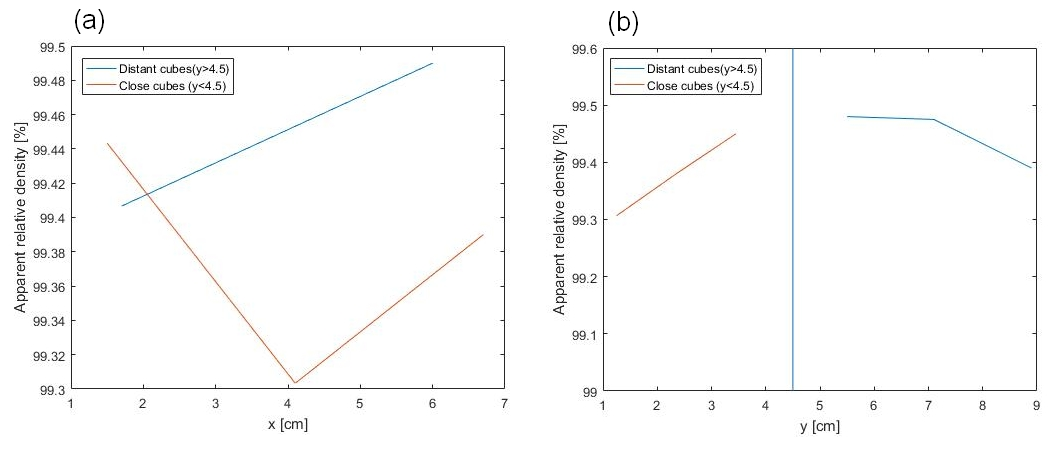
\includegraphics[scale=0.55]{Images/180109-7Dxy}}
\decoRule
\caption[Average apparent relative density of batch X200-180109 type "7" samples as a function of the (a) x coordinate (b) y coordinate]{Apparent relative density of batch X200-180109 type "7" samples as a function of the (a) x coordinate (b) y coordinate}
\label{180109-7Dxy}
\end{figure} 

\begin{figure}[ht]
\centering
\centerline{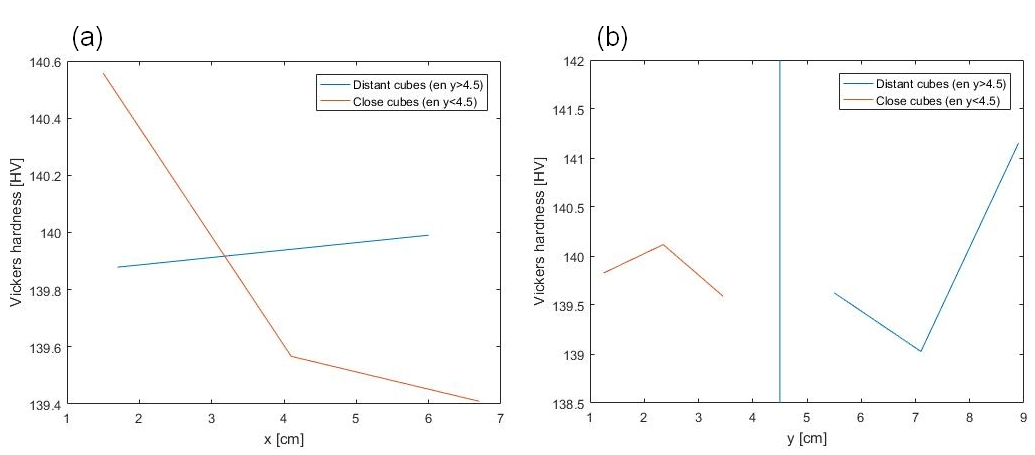
\includegraphics[scale=0.55]{Images/180109-7Hxy}}
\decoRule
\caption[Average Vickers hardness of batch X200-180109 type "7" samples as a function of the (a) x coordinate (b) y coordinate]{Vickers hardness of batch X200-180109 type "7" samples as a function of the (a) x coordinate (b) y coordinate}
\label{180109-7Hxy}
\end{figure} 

\begin{figure}[ht]
\centering
\centerline{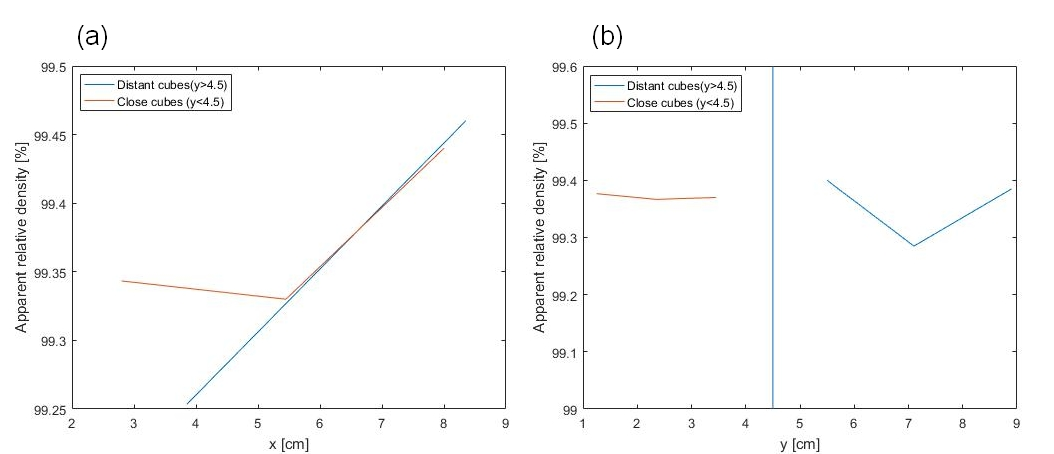
\includegraphics[scale=0.55]{Images/180109-8Dxy}}
\decoRule
\caption[Average apparent relative density of batch X200-180109 type "8" samples as a function of the (a) x coordinate (b) y coordinate]{Apparent relative density of batch X200-180109 type "8" samples as a function of the (a) x coordinate (b) y coordinate}
\label{180109-8Dxy}
\end{figure} 

\begin{figure}[ht]
\centering
\centerline{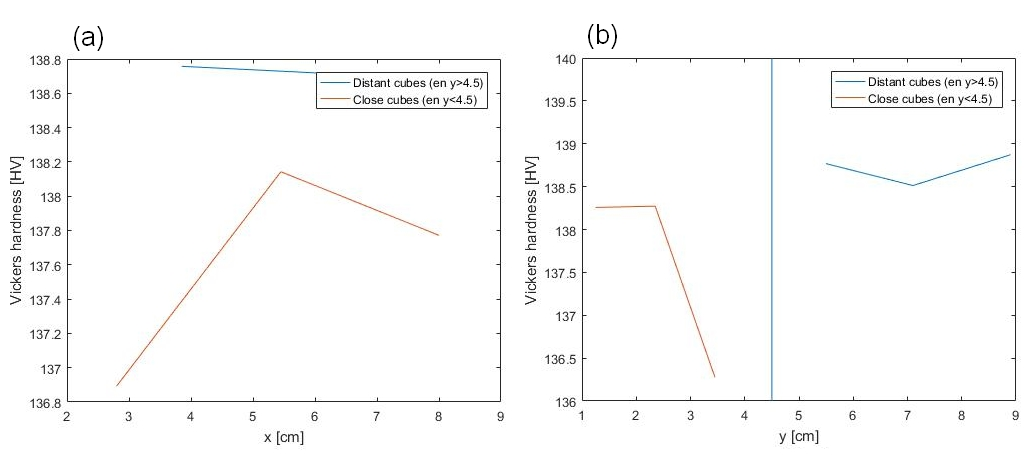
\includegraphics[scale=0.55]{Images/180109-8Hxy}}
\decoRule
\caption[Average Vickers hardness of batch X200-180109 type "8" samples as a function of the (a) x coordinate (b) y coordinate]{Vickers hardness of batch X200-180109 type "8" samples as a function of the (a) x coordinate (b) y coordinate}
\label{180109-8Hxy}
\end{figure} 